\documentclass[letterpaper,addpoints]{exam}
\usepackage{amsmath}
\usepackage{graphicx}
\usepackage{multicol}
\usepackage{pgf}
\usepackage{pgfplots}
\pgfplotsset{compat=1.11}
\usepackage{tikz}
\usepackage{circuitikz}
\usetikzlibrary{arrows,shapes,trees}

\begin{document}

\begin{coverpages}
 \large\bfseries
 
 \noindent 
 Physics 252: Electronics
 
 \vspace{2ex}
 \noindent
 Midterm Exam: March 5, 2015

 \vspace{5ex}
 \noindent 
 Name:\enspace\makebox[2in]{\hrulefill}\\

 \vspace{5ex}
 \noindent 
 This test is administered under the rules and regulations of the honor 
 code of the College of William \& Mary.  

 \vspace{5ex}
 \noindent 
 Show your work, and circle your answers.
 
 \pagebreak
 \vspace{5ex}
 \begin{center}
  \combinedgradetable[v][questions]
 \end{center}
\end{coverpages}
 

\begin{questions}

\begin{question}
 Consider the circuit shown below:
 \begin{center}
  \begin{circuitikz}
   \draw (2.5,0) to[short,o-] (2,0) to[R,l=$R_3$] (0,0) to[battery1,l=$V_{in}$] (0,2) to[R,l=$R_1$] (2,2) to[short,-o] (2.5,2)to[open,v^=$V_{out}$] (2.5,0);
   \draw (0,2) to[R,l=$R_2$,*-*] (2,0);
  \end{circuitikz}
 \end{center}
 where $R_1 = 6$\,k$\Omega$, $R_2 = 6$\,k$\Omega$, $R_3 =3$\,k$\Omega$, and the battery voltage $V_{in} = 18$\,V.
 
 \emph{Hint 1:} For solving the problems below, it may be helpful to mentally connect a load resistor and express symbolically $V_{out}$ versus $I_{out}$ for different values of the load resistors $R_L$.
 \emph{Hint 2:} There is also a faster way that only relies on resistors in parallel and in series.

 \begin{parts}
  \part[4]
  What is the Th\'{e}venin voltage of this circuit?
  \begin{solution}[2in]
  The Th\'{e}venin voltage is the open-circuit voltage.  The open-circuit voltage will be equal to the voltage over resistor $R_2$ in the voltage divider with $R_2$ and $R_3$.  In other words, $V_{Th} = \frac{R_2}{R_2 + R_3} V_{in} = 12\,$V.
  \end{solution}

  \part[5]
  What is the Th\'{e}venin resistance of this circuit?
  \begin{solution}[3.5in]
  The Th\'{e}venin resistance is obtained from the short-circuit current $I_N$.  This is the current through $R_1$ for the circuit with $R_1$ and $R_2$ in parallel, and this combination in series with $R_3$.  The resistance $R_{1\parallel 2}$ is 3\,k$\Omega$, equal to $R_3$, and therefore the voltage across $R_1$ and $R_2$ is half of $V_{in}$ or 9\,V.  The short-circuit current $I_N$ is then 1.5\,mA.  Finally, the Th\'{e}venin resistance is $R_{Th} = \frac{V_{Th}}{I_N} = 8$\,k$\Omega$.
  \end{solution}
  
  \part[5]
  If someone connected a load with resistance $R_L = 4$\,k$\Omega$, what would be the power dissipated by this load?  \emph{Note:} If you are not confident in your results for the previous parts, use $V_{Th} = 8$\,V and $R_{Th} = 12$\,k$\Omega$ and clearly indicate this.
  \begin{solution}[2.5in]
  The voltage across the load will be $V_L = \frac{R_L}{R_L + R_{Th}} V_{Th} = 4$\,V (\emph{2\,V}).  This results in a dissipated power $P_L = \frac{V_L^2}{R_L} = 4$\,mW (\emph{1\,mW}).
  \end{solution}

  \part[6]
  While the same load is connected to the circuit, what is the total power dissipated by all other resistors combined (excluding the load)?  Can you use the Th\'{e}venin equivalent circuit to determine this?
  \begin{solution}[2.5in]
  The total power dissipated in all other resistors is \emph{not} equal to the power generated by the Th\'{e}venin voltage source minus the power dissipated in the load.  We have to use the actual internal circuit.
  \begin{itemize}
  \item The current through the load is $I_L = \frac{V_L}{R_L} = 1$\,mA (\emph{0.5\,mA}).
  \item The voltage across $R_1$ is therefore $V_1 = I_1 R_1 = 6$\,V (\emph{3\,V}) and the power dissipated in $R_1$ is $P_1 = 6$\,mW (\emph{1.5\,mW}).
  \item The voltage across $R_2$ is 10\,V (\emph{5\,V}), the current is $I_2 = \frac{10}{6}$\,mA and the power dissipated is $P_2 = \frac{100}{6}$\,mW (\emph{$\frac{25}{6}$\,mW}).
  \item The current through $R_3$ is $I_3 = I_1 + I_2 = \frac{8}{3}$\,mA (\emph{$\frac{31}{6}$\,mA}) and the voltage across $R_3$ is $V_3 = V_{in} - 10\,\mbox{V} = 8$\,V (\emph{13\,V}), for a power dissipation of $P_3 = \frac{64}{3}$\,mW (\emph{here we see the breakdown of the assumption, since $\frac{V_3}{I_3}$ is not equal to the resistance $R_3$}).
  \end{itemize}
  The total power dissipated is then $P_{1,2,3} = 44$\,mW.
  \end{solution}

 \end{parts}
\end{question}

\pagebreak
\begin{question}
 A circuit consists of a battery with a constant voltage of 2.0\,V, two unknown components and a switch. The switch is closed at $t = 0$ and the output voltage $v_{out}$ across circuit element B is measured as a function of time.
 \begin{multicols}{2}
  \begin{center}
   \begin{circuitikz}[scale=1.5]
    \draw (0,0) node[ground]{} to[battery1,l=$V$] (0,2) to[closing switch,l=switch] (1,2) to[generic,l=A] (3,2) to[short,-o] (3.5,2);
    \draw (0,0) to[short] (3,0) to[short,-o] (3.5,0);
    \draw (3,0) to[generic,l=B,*-*] (3,2);
    \draw (3.5,0) to[open,v>=$v_{out}$] (3.5,2);
   \end{circuitikz}
  \end{center}
 \columnbreak
  \begin{center}
   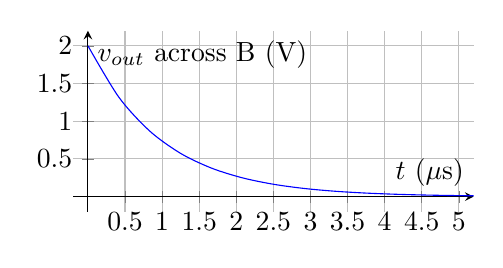
\begin{tikzpicture}
   \begin{axis}[grid=both,
          xlabel=$t$ ($\mu$s),
          ylabel=$v_{out}$ across B (V),
          xtick={0,0.5,1,1.5,2,2.5,3,3.5,4,4.5,5},
          ytick={0,0.5,1,1.5,2},
          xmin=-0.2,ymin=-0.2,
          xmax=5.2,ymax=2.2,
          axis lines=middle,
          height=0.32\textwidth,
          width=0.55\textwidth]
    \addplot[blue,smooth,domain=0:10] {2*pow(e,-x)};
    \end{axis}
   \end{tikzpicture}
  \end{center}
 \end{multicols}
 \begin{parts}
  \part[3]
  What is, based on the graph, the characteristic time of the circuit?
  \begin{solution}[1in]
   The voltage has reached a value of $v(0)e^{-1} = 0.74$\,V after approximately $\tau = 1$\,$\mu$s.
  \end{solution}

  \part[4]
  Sketch the voltage across circuit element A as a function of time.
\begin{center}
 \begin{tikzpicture}[scale=1.0]
  \begin{axis}[grid=both,
          xlabel=$t$ ($\mu$s),
          ylabel=$v_{out}$ across A (V),
          xtick={0,0.5,1,1.5,2,2.5,3,3.5,4,4.5,5},
          ytick={-2,-1.5,-1,-0.5,0,0.5,1,1.5,2},
          xmin=-0.2,ymin=-2.2,
          xmax=5.2,ymax=2.2,
          axis lines=middle,
          height=0.45\textwidth,
          width=0.55\textwidth]
   \ifprintanswers
    \addplot[blue,smooth,domain=0:10] {2*(1-pow(e,-x))};
   \fi
  \end{axis}
 \end{tikzpicture}
\end{center}

  \part[8]
  Draw the diagram for at least two different filter circuits that can produce the observed behavior, \emph{including realistic values for the components}.  In this context ``different circuits'' have at least one component of a different type, so not just a change in values.
  \begin{solution}[2.0in]
   \begin{multicols}{2}
    \begin{center}
     \begin{circuitikz}
      \draw (0,0) node[ground]{} to[battery1,l=$V$] (0,2) to[closing switch,l=switch] (1,2) to[R,l=100\,$\Omega$,o-] (3,2) to[L,l=100\,$\mu$H] (3,0) node[ground]{};
      \draw (3,2) to[short,-o] (4,2) node[right]{$v_{out}$};
     \end{circuitikz}
    \end{center}
   \columnbreak
    \begin{center}
     \begin{circuitikz}
      \draw (0,0) node[ground]{} to[battery1,l=$V$] (0,2) to[closing switch,l=switch] (1,2) to[C,l=10\,nF,o-] (3,2) to[R,l=100\,$\Omega$] (3,0) node[ground]{};
      \draw (3,2) to[short,-o] (4,2) node[right]{$v_{out}$};
     \end{circuitikz}
    \end{center}
   \end{multicols}
  \end{solution}
  
  \part[5]
  With an ohmmeter you measure the equivalent resistance of the two elements as combined in series and you find a value of 100\,$\Omega$.  Which of the two circuits is correct, and what are the values of the two components?
  \begin{solution}[2.5in]
   Since an ohmmeter measures in the low frequency (DC) limit, the circuit must be composed of a resistor and an inductor.  The resistance is 100\,$\Omega$, so the correct solution must be $R = 100\,\Omega$ and $L = 100\,\mu$H.
  \end{solution}
 \end{parts}
\end{question}

\pagebreak
\begin{question}
Consider the circuit diagram in the figure below, with $R = 1$\,k$\Omega$ and a diode-drop voltage $V_d = 0.65$\,V.  The DC input voltage $V_{in}$ is 5\,V.

\begin{center}
 \begin{circuitikz}
  \draw (-2,2) node[left]{$V_{in}$} to[R,l=$R$,o-] (0,2) to[diode,i=$I_d$] (0,0) node[ground]{};
  \draw (0,2) to[short] (1,2) to[R,l=$R$] (1,0) node[ground]{};
  \draw (1,2) to[short,-o] (2,2) node[right]{$V_{out}$};
 \end{circuitikz}
\end{center}

\begin{parts}
\part[4]
What will be the voltage $V_R = V_{in} - V_{out}$ across the resistor connected to the input terminal?
\begin{solution}[2in]
The input voltage $V_{in}$ is large enough to turn on the diode in the forward region.  The voltage across the resistor connected to the input will be one diode-drop less than the input voltage, or $V_R = 4.35$\,V.
\end{solution}

\part[6]
What will be the current $I_d$ through the diode?
\begin{solution}[2in]
The input voltage $V_{in}$ is large enough to turn on the diode in the forward region.  There will therefore be a 0.65\,V voltage over the diode and the resistor connected to ground.  The current through the resistor connected to the input will be 4.35\,mA.  Of this current, 0.65\,mA will go through the resistor connected to ground.  The remaining current will go through the diode, $I_d = 3.70$\,mA.
\end{solution}
\end{parts}
\end{question}

\pagebreak
\begin{question}
 Consider the bridged T-filter shown below.  The input comes in from the left and the output is taken from the right.
 \begin{center}
  \begin{circuitikz}
   \draw (-2,4) node[anchor=east]{$v_{in}$} to[short,o-*] (-1.5,4) to[R,l=$nR$] (1.5,4) to[short,*-o] (2,4) node[anchor=west]{$v_{out}$};
   \draw (-1.5,4) to[short] (-1.5,3) to[C,l=$C$] (0,3) to[C,l=$C$] (1.5,3) to[short] (1.5,4);
   \draw (0,3) to[R, l=$R/n$, *-] (0,1) node[ground]{};
  \end{circuitikz}
 \end{center}
 \begin{parts}
  \part[4]
   What is the magnitude of the gain of this circuit for very low frequencies?
   \begin{solution}[2.5in]
    At low frequencies, the capacitors act as open circuits, and the filter circuit is completely disconnected from ground.  The output voltage will be identical to the input voltage.  Thus, $|G(\omega\to 0)| = 1$.
   \end{solution}
   
  \part[4]
   What is the magnitude of the gain of this circuit for very high frequencies?
   \begin{solution}[2.5in]
    At high frequencies, the capacitors act as shorts, and the input terminal is connected directly to the output terminal.  Thus, $|G(\omega\to\infty)| = 1$.
   \end{solution}
   
   \part[2]
   What type of filter can this be, based on your answers above?
   \begin{solution}[1in]
    Since the filter has unity gain in both the low frequency and high frequency limit, it must be a band reject filter or a band-pass amplifier.
   \end{solution}

  \bonuspart[10]
   What is the gain of this circuit at $\omega_{RC} = \frac{1}{RC}$ when $n = 2$? \emph{Hint 1:} A straight-forward but tedious approach is to use Kirchhoff's rules. \emph{Hint 2:} A faster approach is to use voltage dividers to determine $G(\omega)$.
  \begin{solution}[4.0in]
   The output voltage can be written as $v_{out} = v_{in} - v_{nR}$.  We can find $v_{nR}$ by using the voltage divider equation twice:
   \begin{eqnarray*}
   v_{nR} & = & v_{in} \frac{\frac{1}{j\omega C} \parallel (nR + \frac{1}{j\omega C})}{R/n + \frac{1}{j\omega C} \parallel (nR + \frac{1}{j\omega C})} \frac{nR}{nR + \frac{1}{j\omega C}} \\
   & = & v_{in} \frac{\frac{1}{j\omega C} (nR + \frac{1}{j\omega C})}{R/n (\frac{1}{j\omega C} + nR + \frac{1}{j\omega C}) + \frac{1}{j\omega C} (nR + \frac{1}{j\omega C})} \frac{nR}{nR + \frac{1}{j\omega C}} \\
   & = & v_{in} \frac{nR + \frac{1}{j\omega C}}{R/n (2 + j\omega n R C) + (nR + \frac{1}{j\omega C})} \frac{j \omega n R C}{j \omega n R C + 1} \\
   & = & v_{in} \frac{j \omega n R C + 1}{j \omega R C /n (2 + j \omega n R C) + (j \omega n R C + 1)} \frac{j \omega n R C}{j \omega n R C + 1} \\
   & = & v_{in} \frac{j \omega n R C}{j \omega R C /n (2 + j \omega n R C) + (j \omega n R C + 1)}.
   \end{eqnarray*}
   This results in the following expression for the gain:
   \begin{eqnarray*}
    G(\omega) & = & \frac{v_{out}}{v_{in}} = 1 - \frac{v_{nr}}{v_{in}} \\
    & = & 1 - \frac{j \omega n R C}{j \omega R C /n (2 + j \omega n R C) + (j \omega n R C + 1)} \\
    & = & \frac{j \omega R C /n (2 + j \omega n R C) + 1}{j \omega R C /n (2 + j \omega n R C) + (j \omega n R C + 1)} \\
    & = & \frac{1 + j \omega R C (2 / n) - \omega^2 (R C)^2}{1 + j \omega R C (2 / n + 1) - \omega^2 (R C)^2}.
   \end{eqnarray*}
   At $\omega_{RC} = 1/RC$ this results in a magnitude of
   \begin{equation*}
    |G(\omega_{RC})| = \frac{2 / n}{2 / n + 1} = \frac{1}{2} \mbox{ for } n=2
   \end{equation*}
  \end{solution}
 
 \end{parts}
\end{question}

\end{questions}

\end{document}
g